%\chapter{Reo} \label{chapter:reo}
%In this chapter, a succinct overview of Reo~\cite{Arbab2004,Arbab2006} is presented, considering its main characteristics with two usage examples. We also briefly introduce the main aspects of one popular formal semantics for Reo, Constraint Automata as proposed by Baier et al.~\cite{Baier2006}. We also introduce two usage examples of Reo, which will later be discussed in Chapter~\ref{chap:reloApproach}, bound to show how one can formalize and certify Reo circuits employing \relo.

%\subsection{Reo} \label{sec:reo}
% -> ERICK: 14/11/2021 - seção foi mergeada com a seção de related work
%%Reo~\cite{Arbab2004,Arbab2006} is a graphic-based coordination modelling language based on channels where complex coordinators are compositionally built from simpler ones. These complex coordinators are called connectors and compose the very heart of Reo. 
%
%In this section, we provide a succinct overview of Reo~\cite{Arbab2004,Arbab2006}, considering its main characteristics with two usage examples. We also briefly introduce the main aspects of one popular formal semantics for Reo, Constraint Automata as proposed by Baier et al.~\cite{Baier2006}. %We also introduce two usage examples of Reo, which will later be discussed in Chapter~\ref{chap:reloApproach}, bound to show how one can formalize and certify Reo circuits employing \relo.


\subsection{The Reo Modelling Language} \label{sec:reo}
%In recent years, many software developers have researched new techniques on how to develop software. Technologies and methods have emerged since the nineties, such as service-oriented computing~\cite{Papazoglou2003} and model-driven development~\cite{Atkinson2003}, where the first one advocates the idea of composing software out of other software and the latter, developing software based on previous models.%

%Reo~\cite{Arbab2004,Arbab2006} is a graphic-based coordination modelling language based on channels where complex coordinators are compositionally built from simpler ones. These complex coordinators are called connectors and compose the very heart of Reo.% 

%The behavior modelled by these connectors provide essentially the model of the ``glue-code'', the code which coordinates how connected entities in the model interact with each other. Hence, Reo is conceived as a language that eases the modelling of interaction between instances (software abstractions) of different components that acts together in a component-based system.

%The usage of channel-based models is considered an alternative to advocate model-driven development of such ``glue code``. A Reo channel is an entity that connects two distinct ends with its own unique behavior. Channels can be seen as primitives for modelling concurrent systems. The usage of channel-based models brings a number of advantages by efficiently modelling primitives of concurrent systems (remote function calls, message passing and shared memory, to name a few), enabling the capture of properties like efficiency of how messages are exchanged and safety of how data can be inadvertently used by other entities in other modelling paradigms (such as shared data space modelling) by the model, a situation that does not occur in point-to-point communication.%

%o parágrafo abaixo tava abaixo do parágrafo que começa com "As a coordination model, Reo focuses"
%Reo plays a central role in integrating software components, especially considering Component-Based Software Engineering, where it is expected that software components are independent of each other, being more adapted to the environment they were conceived for. In recent times, software development has shifted from building large, single instances of a system to building systems by reuse of already existing pieces of software, where the full application (system) itself is generated through the orchestrated interaction of these software components, where Reo may be adequate in orchestrating such interaction.

As a coordination model, Reo focuses on connectors, their composition, and how they behave, not focusing on particular details regarding the entities that are connected, communicate, and interact through those connectors. Connected entities may be modules of sequential code, objects, agents, processes, web services, and any other software component where its integration with other software can be used to build a system~\cite{Arbab2004}. Such entities are defined as component instances in Reo.

%The notion of Reo as an integrator between different instances of software component is further explored in the following idea: in Component Based Software Engineering, software components are expected to be independent from each other and more adapted to the environment they are meant to act on. Nowadays, software development is shifting from rather big, single instances of a system to reusable services, in order to produce a full application. This is the very heart of service-oriented computing, where such services can be modules, systems, web services or any other self-contained piece of loosely coupled software.

%However, if the software development process considers the integration of such services by means of data exchange between their interfaces, the core of this data exchange (the specification of how such exchange happens) must be left out of each component in order to maintain software construction by (re)using seamless integration of existing services. Therefore a specific "glue-code`` must be written for each built software. %Reo excels at modelling such interaction, advocating the very heart of service-oriented computing.

%Theoretically, service-oriented computing is analogue to exogenous coordination, where the coordination is done "externally`` from the system's point of view, advocating the idea of separating the computation offered by integration of different, multiple services from how they integrate (the coordination of its data exchange) with each other~\cite{Arbab1996}. Reo propagate such principles by providing out-of-the-box concepts and tools to develop the "glue-code`` that acts as the coordinator of services' integration, given how they interact with their respective environment.

%Component instances are defined as a non-empty set $P$ that denotes a set of entities involved in an instance (process, services, actors, usually denoted by capital letters) and a predefined set of I/O operations associated with each of those entities, where they only interact with each other by the channel that connects these instances. A software component is a software implementation that may execute in physical or logical devices. Therefore, software components are abstract entities that describe the behavior of its instances.

%A system in Reo is composed by instances of software component that interacts with each other by means of Reo connectors. Component instances are defined as a non-empty set $P$ that denotes a set of entities involved in an instance (process, services, actors) and a predefined set of I/O operations associated with those entities where the only means of performing such operations are through channel ends connected to this set. A software component is a software implementation which may execute in physical or logical devices. Therefore, software components are abstract entities that describes the behavior of its instances.

Channels in Reo are defined as a point-to-point link between two distinct nodes, where each channel has its unique predefined behavior. Each channel in Reo has exactly two ends, which can be of the following types: the source end, which accepts data into the channel, and the sink end, which dispenses data out of the channel. Channels are used to compose more complex connectors, being possible to combine user-defined channels amongst themselves and with the canonical connectors provided by Baier et al.~\cite{Baier2006}. Figure~\ref{fig:reoCanonical} shows the basic set of connectors as presented by Kokash et al.~\cite{Kokash2012}. %Table~\ref{tab:reoConnectors} relates the canonical Reo connectors with their behavior.

\usetikzlibrary{snakes}	
\begin{figure*}[!htb] 
	\centering\subfigure[Sync]{	
		\centering \begin{tikzpicture}[->,>=stealth',font=\sffamily,semithick,node distance=1.8cm]
		\node (A)  {$A$};
		\node (B) [right of=A]  {$B$};
		\path (A) edge  node {} (B);
		
		\end{tikzpicture}
	}\quad
	\subfigure[LossySync]{
		\centering \begin{tikzpicture}[->,>=stealth',font=\sffamily,semithick,node distance=1.8cm,dashed]
		\node (A)  {$A$};
		\node (B) [right of=A]  {$B$};
		\path (A) edge  node {} (B);
		
		\end{tikzpicture}
	}\quad
	\subfigure[FIFO]{
		\centering 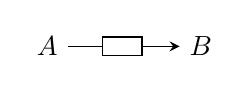
\begin{tikzpicture}[->,>=stealth,font=\sffamily,semithick,node distance=1cm]
		\node (A)  {$A$};
		\node (x) [draw,rectangle,minimum width=0.5cm,minimum height=0.2cm] at  (.95,0) {}; %[draw=black,rectangle,inner sep=5pt] at  (.88,0) {} ;
		%\node (x) [circle,fill,inner sep=1pt,right of=A] {};
		%\node (y) [circle,fill,inner sep=1pt,right of=x] {};
		\node (B) [right of=x]  {$B$};
		\draw[semithick,-] (A) -- ++(.7cm,0) |- (.5,0);
		\draw [semithick,->](x) edge  node {} (B);
		
		\end{tikzpicture}	
	}
	\subfigure[SyncDrain]{
		\centering 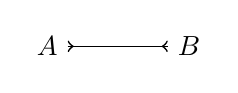
\begin{tikzpicture}[->,>=to reversed,font=\sffamily,semithick,node distance=1.8cm]
		\node (A)  {$A$};
		\node (B) [right of=A]  {$B$};% 2cm below, 1cm to the left (optional)
		\path (A) edge  node {} (B)
		(B) edge  node {} (A);
		
		\end{tikzpicture}	
	}\quad
	\subfigure[AsyncDrain]{
		\centering 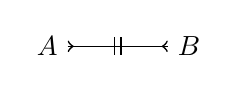
\begin{tikzpicture}[->,>=to reversed,font=\sffamily,semithick,node distance=1.8cm]
		\node (A)  {$A$};
		\node (B) [right of=A]  {$B$};
		\path (A) edge  node {\tikz \draw[|-|,semithick ] (0,0) -- +(.1,0);} (B)
		(B) edge  node {} (A);
		
		\end{tikzpicture}	
	}
	
	\subfigure[\mbox{Filter}]{
		\centering 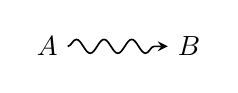
\begin{tikzpicture}[->,decorate,decoration=snake,>=stealth,font=\sffamily,semithick,node distance=1.8cm]
		\node (A)  {$A$};
		\node (B) [right of=A]  {$B$};
		%\path (A) edge  node (B);%{\tikz \draw [->,decorate,decoration=snake] (0,0) -- +(.1,0);} (B);
		\draw [->,decorate,decoration=snake] (A) -- (B);
		\end{tikzpicture}	
	}\quad
	\subfigure[\mbox{Transform}]{
		\centering \begin{tikzpicture}[->,>=stealth,font=\sffamily,semithick,node distance=1.8cm,]
		\node (A)  {$A$};
		%\node (x) [draw,triangle 90] at  (.88,0) {};
		\node (B) [right of=A]  {$B$};% 2cm below, 1cm to the left (optional)
		%\draw[semithick,-] (A) -- ++(.7cm,0) |- (.5,0);
		%\draw [semithick,->](x) edge  node {} (B);
		\path (A) edge node {\tikz \draw[-triangle 90,] (0,0) -- +(.1,0);} (B);
		
		\end{tikzpicture}	
	}\quad
	\subfigure[Merger]{
		\centering 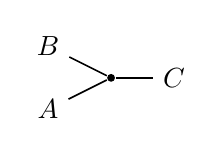
\begin{tikzpicture}[>=stealth,font=\sffamily,semithick,node distance=.8cm]
		\node (A) at (0,0) {$A$};
		\node (B) at (0,0.8)  {$B$};
		\node (x) [fill,circle,inner sep=1pt] at (0.8,0.4) {};
		\node (C) [right of=x] {$C$};
		\path (A) edge  node {} (x)
		(B) edge  node {} (x)
		(x) edge  node {} (C); %[->,thick,font=\sffamily,>=stealth] node {} (C);
		
		\end{tikzpicture}	
	}\quad
	\subfigure[\mbox{Replicator}]{
		\centering 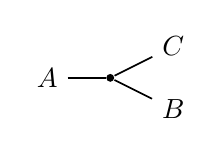
\begin{tikzpicture}[>=stealth,font=\sffamily,semithick,node distance=1cm]
		\node (A) {$A$};
		\node (x) [fill,circle,inner sep=1pt] at (0.8,0) {}; %[fill,circle,inner sep=1pt] at (0.8,0.4) {};
		\node (B) at (1.6,-0.4) {$B$};
		\node (C) at (1.6,0.4)  {$C$};
		\path (A) edge  node {} (x)
		(x) edge  node {} (B)
		(x) edge node  {} (C);
		%(x) edge[->,thick,font=\sffamily,>=stealth] node {} (C);
		
		\end{tikzpicture}	
	}
	\caption{Canonical Reo connectors}
	\label{fig:reoCanonical}
\end{figure*}

%\begin{table}[!htb]
%	
%	\centering\begin{tabular}{p{2cm} | p{2.6cm} | p{9cm} }
%		\toprule
%		Connector & Reo & Behaviour \\\midrule
%		
%		Sync & \begin{tikzpicture}[->,>=stealth',font=\sffamily,semithick,node distance=1.8cm]
%		\node (A)  {$A$};
%		\node (B) [right of=A]  {$B$};
%		\path (A) edge  node {} (B);
%		
%		\end{tikzpicture} & Data flows Synchronously from $A$ to $B$.  \\\midrule
%		
%		LossySync & \begin{tikzpicture}[->,>=stealth',font=\sffamily,semithick,node distance=1.8cm,dashed]
%		\node (A)  {$A$};
%		\node (B) [right of=A]  {$B$};
%		\path (A) edge  node {} (B);
%		
%		\end{tikzpicture} & Data either flows Synchronously from $A$ to $B$, or it is lost in its way from $A$ to $B$ due so some communication faliure (i.e., link failure between the interfaces).  \\\midrule
%		
%		FIFO & \begin{tikzpicture}[->,>=stealth,font=\sffamily,semithick,node distance=1cm]
%		\node (A)  {$A$};
%		\node (x) [draw,rectangle,minimum width=0.5cm,minimum height=0.2cm] at  (.95,0) {}; %[draw=black,rectangle,inner sep=5pt] at  (.88,0) {} ;
%		%\node (x) [circle,fill,inner sep=1pt,right of=A] {};
%		%\node (y) [circle,fill,inner sep=1pt,right of=x] {};
%		\node (B) [right of=x]  {$B$};
%		\draw[semithick,-] (A) -- ++(.7cm,0) |- (.5,0);
%		\draw [semithick,->](x) edge  node {} (B);
%		
%		\end{tikzpicture} & Data flows from $A$ to $B$ in a buffer-fashioned manner. It first leaves $A$, then it is stored in a intermediate place before reaching $B$. \\\midrule
%		
%		SyncDrain & \begin{tikzpicture}[->,>=to reversed,font=\sffamily,semithick,node distance=1.8cm]
%		\node (A)  {$A$};
%		\node (B) [right of=A]  {$B$};% 2cm below, 1cm to the left (optional)
%		\path (A) edge  node {} (B)
%		(B) edge  node {} (A);
%		
%		\end{tikzpicture} & The data flow of $A$ and $B$ must be synchronized. \\\midrule
%		
%		AsyncDrain & \begin{tikzpicture}[->,>=to reversed,font=\sffamily,semithick,node distance=1.8cm]
%		\node (A)  {$A$};
%		\node (B) [right of=A]  {$B$};
%		\path (A) edge  node {\tikz \draw[|-|,semithick ] (0,0) -- +(.1,0);} (B)
%		(B) edge  node {} (A);
%		
%		\end{tikzpicture} & The data flow of $A$ and $B$ must not be synchronized. \\\midrule
%		
%		Filter & \begin{tikzpicture}[->,decorate,decoration=snake,>=stealth,font=\sffamily,semithick,node distance=1.8cm]
%		\node (A)  {$A$};
%		\node (B) [right of=A]  {$B$};
%		%\path (A) edge  node (B);%{\tikz \draw [->,decorate,decoration=snake] (0,0) -- +(.1,0);} (B);
%		\draw [->,decorate,decoration=snake] (A) -- (B);
%		\end{tikzpicture} & A data item $d$ will successfully be transmitted from $A$ to $B$ if it satisfies a logical predicate $P$. \\\midrule
%		
%		Transform & \begin{tikzpicture}[->,>=stealth,font=\sffamily,semithick,node distance=1.8cm,]
%		\node (A)  {$A$};
%		%\node (x) [draw,triangle 90] at  (.88,0) {};
%		\node (B) [right of=A]  {$B$};% 2cm below, 1cm to the left (optional)
%		%\draw[semithick,-] (A) -- ++(.7cm,0) |- (.5,0);
%		%\draw [semithick,->](x) edge  node {} (B);
%		\path (A) edge node {\tikz \draw[-triangle 90,] (0,0) -- +(.1,0);} (B);
%		
%		\end{tikzpicture} & A data item $d$ will be transformed by a transformation function $f\colon data \to data$ before reaching $B$. \\\midrule
%		
%		Merger & \begin{tikzpicture}[>=stealth,font=\sffamily,semithick,node distance=.8cm]
%		\node (A) at (0,0) {$A$};
%		\node (B) at (0,0.8)  {$B$};
%		\node (x) [fill,circle,inner sep=1pt] at (0.8,0.4) {};
%		\node (C) [right of=x] {$C$};
%		\path (A) edge  node {} (x)
%		(B) edge  node {} (x)
%		(x) edge  node {} (C); %[->,thick,font=\sffamily,>=stealth] node {} (C);
%		
%		\end{tikzpicture} & The data from ports $A$ and $B$ are transmitted to $C$ similar to the functioning of a demultiplex \\\midrule
%		
%		Replicator & \begin{tikzpicture}[>=stealth,font=\sffamily,semithick,node distance=1cm]
%		\node (A) {$A$};
%		\node (x) [fill,circle,inner sep=1pt] at (0.8,0) {}; %[fill,circle,inner sep=1pt] at (0.8,0.4) {};
%		\node (B) at (1.6,-0.4) {$B$};
%		\node (C) at (1.6,0.4)  {$C$};
%		\path (A) edge  node {} (x)
%		(x) edge  node {} (B)
%		(x) edge node  {} (C);
%		%(x) edge[->,thick,font=\sffamily,>=stealth] node {} (C);
%		
%		\end{tikzpicture} & Data from $A$ is simutaneously replicated to $B$ and $C$, similar to a multiplex. \\\bottomrule
%	\end{tabular}
%	\caption{Basic Reo channels and their behaviour}
%	\label{tab:reoConnectors}
%\end{table}

%A node in Reo is defined as a logical structure denoting how channel ends are linked to each other in Reo connectors.
%Nodes composing channel ends in Reo can be either source nodes, sink nodes, or mixed nodes. Source nodes are nodes that accept data into the channel, i.e., nodes that serve as a gateway to data flow into the channel, while sink nodes are nodes where data flows out of the channel and mixed nodes are nodes that act both as source nodes and sink nodes. 

Channel ends can be used by any entity to send/receive data, given that the entity belongs to an instance that knows these ends. Entities may use channels only if the instance they belong to is connected to one of the channel ends, enabling either sending or receiving data (depending on the kind of channel end the entity has access to).

The bound between a software instance and a channel end is a logical connection that does not rely on properties such as the location of the involved entities. Channels in Reo have the sole objective to enable the data exchange following the behaviour of the connectors composing the channel, utilizing I/O operations predefined for each entity in an instance. A channel can be known by zero or more instances at a time, but its ends can be used by at most one entity at the same time. %Both channels and software components can be mobile entities. Since Reo is not interested in specific details of a software instance (only on how it interfaces with the outside world), this leads to the possibility of the configuration of Reo connectors to change dynamically. 

%The mobility of Reo channels and instances does not affect the connections of instances and channels, which only depends on the instance's will to connect to (or disconnect from) channel ends. This idea reflects the idea that, unrelated with their location, a software instance may be connected to another software instance while moving or after moving from its original location to elsewhere, where the channel only provides the medium of how they interact with each other. 

%\begin{figure} \label{fig:reoCanonical}
%\centering \includegraphics[scale=0.68]{images/reoConnectors}
%\caption{Canonical set of Reo channels as provided by \cite{Kokash2009}}\bruno{Crie suas próprias figuras.}
%\end{figure}

%\begin{figure}
%\begin{subfigure}[Sync]	
%\centering \begin{tikzpicture}[->,>=stealth',font=\sffamily,semithick]%,node distance=1.8cm]
%\node (A) at (0,0) {$A$};
%\node (x) [circle,fill,inner sep=1pt] at (0,1) {};
%\node (y) [circle,fill,inner sep=1pt,right of=x] {};
%\node (B) [right of=y]  {$B$};% 2cm below, 1cm to the left (optional)
%\path (x) edge node {} (y);%[->,thick,stealth]  node {} (B);
%\end{tikzpicture}
%\end{subfigure}

Figure~\ref{fig:SequencerReo} introduces a Reo connector known as Sequencer\footnote{\url{http://arcatools.org/reo}}. It models the data flow between three entities sequentially. The data flows from the first FIFO connector (a buffer), which will be sequentially synchronized with entities in port names names A, B, and C. The Sequencer can be used to model scenarios where processes sequentially interact between themselves.

\begin{figure}[!htb] 
	\centering %\scalebox{0.73}[0.73]{
		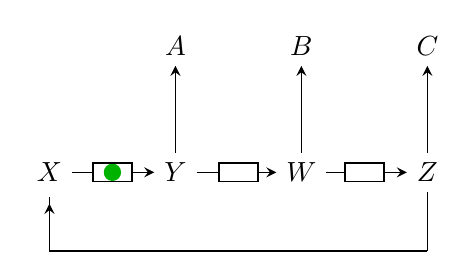
\begin{tikzpicture}[>=stealth,font=\sffamily,semithick,node distance=1.6cm]
		\node (bo1) [draw,scale=0.6,fill,circle,color=green!70!black] at (1.2,-1.5) {};
		\node (A) [] at (0.4,-1.5) {$X$};
		\node (y) [] at (2,-1.5) {$Y$};
		\node (B) [above of = y] {$A$};
		\node (x) [draw,rectangle,minimum width=0.5cm,minimum height=0.2cm] at (1.2,-1.5) {};
		\node (z) [draw,rectangle,minimum width=0.5cm,minimum height=0.2cm] at (2.8,-1.5) {};
		\node (a) [] at (3.6,-1.5) {$W$};
		\node (C) [above of = a] {$B$};
		\node (b) [] at (5.2,-1.5) {$Z$};
		\node (c) [draw,rectangle,minimum width=0.5cm,minimum height=0.2cm] at (4.4,-1.5) {};
		\node (D) [above of = b] {$C$};
		\draw[semithick,-] (b) -- ++(0,-0.5) |- (5.2,-2.5);
		\draw[semithick,-] (5.2,-2.5) -- ++(0,0) |- (0.4,-2.5);
		\draw[semithick,->] (0.4,-2.5) |- (0.4,-1.9);	
		\path (A) edge[-] node{} (x)
		(x) edge[->] node{} (y)
		(y) edge[->] node{} (B)
		(y) edge[-] node{} (z)
		(z) edge[->] node{} (a)
		(a) edge[->] node{} (C)
		(a) edge[-] node{} (c)
		(c) edge[->] node{} (b)
		(b) edge[->] node{} (D);
		\end{tikzpicture}
	%}
	\caption{Modelling of the Sequencer in Reo}%\bruno{Melhor remover o ``ponto'' verde}}
	\label{fig:SequencerReo}
\end{figure}

%Figure~\ref{fig:bigCircuit} models a simplification of a scenario containing two Smart traffic lights $A$ and $B$ in a crossroad. Their default functioning follows a timed schedule: while one of them is green, the other is red. In addition to this timed behaviour, a controlling station has a sensor (i.e., a camera, denoted by the upper dot) that monitors the crossroad and identifies whether there is heavy traffic waiting for the green light on one of the traffic lights~\cite{Grilo2020}. %Figure~\ref{fig:bigCircuit} models the described scenario as a Reo circuit.
%%\erick{We collapse the destination of $P$ and $\neg P$ for space limitations as the following should be the same (one circuit for each semaphore of the cross). - entendo que essa frase deverá ser removida.}
%
%Intuitively, the circuit controls the effective time a traffic light may be green or red depending on the number of cars waiting to pass. This may be done by verifying which data item is coming from both the timer and the sensor, and when is these data incoming. The circuit filters this data, to mutually exclude one of the traffic lights. The destination node (denoted by the leftmost dot in Figure~\ref{fig:bigCircuit}) will receive the data item (0 or 1) and, based on this item decide which traffic light gains the priority to go green. 

%Figure~\ref{fig:bigCircuit} models a circuit where data is interchanged and alternated (e.g, a semaphore). The data incoming from the uppermost dot denotes a property which the sensor has detected (i.e., many cars waiting for the traffic light to be green), while $d$ is a data item denoting that the semaphores will alternate between open and closed, enabling the interchange of which traffic light will be either open or closed (the interchange between $d$ and $!d$ forced by the circuit renders unable the scenario where one of the traffic lights is always open). The leftmost node denotes the sink node where the data sent by the sensors enters the circuit.
%
%\begin{figure}[!htb]
%	\centering
%	\begin{tikzpicture}[rotate=90,transform shape, >=stealth,font=\sffamily,semithick,node distance=1.3cm]
%	\node (Ctrl) [fill,circle,inner sep=1pt] at (-2,0){};
%	%\node (x) [fill,circle,inner sep=1pt] at (-0.8,0) {}; %[fill,circle,inner sep=1pt] at (0.8,0.4) {};
%	%\node (A) [fill,circle,inner sep=1pt] at (-1.6,-0.4) {};
%	%\node (B) [fill,circle,inner sep=1pt] at (-1.6,0.4)  {};
%	%\node (Af1) [fill,circle,inner sep=1pt,left of=A]  {};%filter de baixo
%	%\node (Af2) [fill,circle,inner sep=1pt,left of=B]  {};%filter de cima
%	\node (Syn1) [fill,circle,inner sep=1pt,left of=B] at (-2.4,0) {};
%	\node (Timer) [fill,circle,inner sep=1pt,below of=Syn1] {};
%	\node (labelTimer) at (-3.4,-1.4) {$A/B$};
%	%segundo replicator
%	\node (y) [fill,circle,inner sep=1pt,above of=Syn1] {}; %[fill,circle,inner sep=1pt] at (0.8,0.4) {};
%	\node (Rep1) [fill,circle,inner sep=1pt] at (-4.2,2.2) {};
%	\node (Rep2) [fill,circle,inner sep=1pt] at (-3.3,2.2)  {};
%	%os dois transformers (alô optimus)
%	\node (Trsf1) [fill,circle,inner sep=1pt,above of = Rep1] {};
%	\node (label) at (-4.6,2.85) {$!d$};
%	\node (Trsf2) [fill,circle,inner sep=1pt, above of=Rep2]  {};
%	\node (Endp1) [fill,circle,inner sep=1pt] at (-3.8,4.8)  {};
%	%	%sensor novo --- mais a direita la em cima
%	%	\node (FifoIn) [fill,circle,inner sep=1pt,right of= Endp1] at (-3.9,3.5) {};
%	%	\node (Ctrl2) [fill,circle,inner sep=1pt,right of= FifoIn] at (-2.7,3.5)  {};
%	%	\node (labelC) at (-1.2,3.5)  {$C$};
%	%	\node (FifoOut) [fill,circle,inner sep=1pt,above of= Ctrl2] at (-3.0,3.45) {};
%	%	%merger mais acima
%	%	\node (mergerP1) [fill,circle,inner sep=1pt] at (-3.5,5.7) {};
%	
%	
%	%sumidouro do conector --- ele é mesmo necessário?
%	\node (Final) [inner sep=1pt,above of =Endp1] {$C$};%,left of= Endp1] {}; %at (-3.5,5.5) {};
%	%\path (A) edge  node (B);%{\tikz \draw [->,decorate,decoration=snake] (0,0) -- +(.1,0);} (B);
%	%\draw [->,decorate,decoration=snake] (B) -- (Af2) node[midway,above] {$P(x)$};
%	%\draw [->,decorate,decoration=snake] (A) -- (Af1) node[midway,below] {$\neg P(x)$};
%	\node (rec) [draw,rectangle,minimum width=0.4cm,minimum height=0.2cm,rotate = 110] at  (-3.45,4.15) {}; 
%	%retangulo do fifo "solto"
%	%\node (rec2) [draw,rectangle,minimum width=0.4cm,minimum height=0.2cm,rotate = 110] at  (-2.8,4.1) {}; 
%	\path (Ctrl) edge [semithick,->] node {} (Syn1)%(x)
%	%(x) edge [semithick,->]  node {} (A)
%	%(x) edge [semithick,->] node  {} (B)
%	%(Af1) edge [semithick,->] node {} (Syn1)
%	%(Af2) edge [semithick,->] node {} (Syn1)
%	(Timer) edge [semithick,->] node {} (Syn1)
%	(Syn1) edge [semithick,->] node {} (y)
%	(y) edge [semithick,->] node {} (Rep1)
%	(y) edge [semithick,->] node {} (Rep2)
%	(Rep1) edge node {\tikz \draw[-triangle 90,rotate = 90] (0,0) -- +(.1,0);} (Trsf1)
%	(Rep2) edge [semithick,->,align=center,right] node {$d$} (Trsf2)
%	(Trsf1) edge [semithick,->,align=center] node {} (Endp1)
%	(Trsf2) edge [semithick,align=center] node {} (rec)
%	(rec) edge [semithick,->,align=center] node {} (Endp1)
%	(Endp1) edge [semithick,->,align=center] node {} (Final);
%	%	(Endp1) edge [semithick,->,align=center] node {} (mergerP1);
%	%	\path (Ctrl2) edge [semithick,->,align=center] node {} (FifoIn)
%	%	(FifoIn) edge [semithick,-,align=center] node {} (rec2)
%	%	(rec2) edge [semithick,->,align=center] node {} (FifoOut)
%	%	(FifoOut) edge [semithick,->,>=to reversed]  node {} (Endp1)
%	%	(Endp1) edge  [semithick,->,>=to reversed] node {} (FifoOut)
%	%	(FifoOut) edge [semithick,->,align=center] node {} (mergerP1)
%	%	(mergerP1) edge [semithick,->,align=center] node {} (Final);
%	\end{tikzpicture}
%	\caption{A Reo model for smart traffic lights and a controller of a crossroad}
%	\label{fig:bigCircuit}
%\end{figure}

%Reo can also be used to model a consensus algorithm that deals with Byzantine fault~\cite{Lamport1982} to achieve consensus under uncertainty, which may be caused by different factors (varying from network issues to faulty agents). Intuitively, these machines can lead to ``bad decisions'' to be taken in a consensus-based distributed system. Among the algorithms conceived to address this problem, the delegated Byzantine Fault Tolerance 2.0 (dBFT)~\cite{Neo2015} was employed for the Neo Blockchain to achieve consensus globally in the system. It takes quorum-based decisions in an environment with $3f + 1$ machines, where at most $f$ machines can present Byzantine fault-like behavior. A machine in dBFT is also called a replica.

%ERICK: 02/11 - Só faz sentido explicar o byzantine fault se for usar ele
%The dBFT 2.0 is an algorithm split into three steps: I) One of the replicas
%will be chosen as the primary, being responsible to propose an information pack, II) the remainder of the replicas (known as backups) will validate such information, and III) finally commit to that information, as soon as $2f+1$ valid responses are available. After commitment, the replica is unable to revert its own decision, so the logic ensures that each local commit decision, once made
%by an honest replica, will represent a global commit after passing the uncertain quorum $2f + 1$ threshold. If enough time passes without changing state (assuming that the primary system may have failed), then a condition is triggered that will reset the whole process and restart from the next primary. This process is known as view change.

%Figure~\ref{fig:byzantineFaultReo} models the communication structure of a replica in dBFT in Reo. Node A' denotes the circuit data input, which will be filtered to the primary node P or backup node B in a round-robin scheme as follows:
%
%\begin{itemize}
%	\item  If the data flows from A to node P, after a preset time the data flow from P to the request node R. From R, there are two accessible nodes: one that will timeout after a preset time and will put the machine in the change view node V' (by flowing data from R to V'); and one that will move the system to the commit node CA' if the test condition for the validity of the block passes (by flowing data from R to C'). 
%	
%	\item If the data flow from A to node B, after a preset time it will move to the change view node VR'. Node R' represents other replicas in the network, where its data will be the requests released by the other consensus replicas, which arrive in R' with a bounded nondeterministic delay. All filters in the model that have their sink node one of the V' nodes denote the preset time the replica will wait to change its state to change view (V').
%\end{itemize}

%\begin{figure}[!htb] 
%	\centering \scalebox{0.83}[0.83]{
%		\begin{tikzpicture}[transform shape, >=stealth,font=\sffamily,semithick,node distance=1.3cm]
%		\node (A) [fill,circle,inner sep=1.5pt]{};
%		\node (B) [fill,circle,inner sep=1.5pt, right of=A]{};
%		%\node (Bt) [fill,circle,inner sep=1pt, right of=B] at (0.6,0) {};
%		\node (C) [fill,circle,inner sep=1.5pt, right of=B]{};
%		\node (D) [fill,circle,inner sep=1.5pt, right of=C]{};
%		%\node (Dt) [fill,circle,inner sep=1pt, right of=D] at (3.2,0) {};
%		\node (F) [fill,circle,inner sep=1.5pt, right of=D]{};
%		\node (E) [fill,circle,inner sep=1.5pt, below of=D]{};
%		\node (G) [fill,circle,inner sep=1.5pt, right of=E]{};
%		\node (H) [fill,circle,inner sep=1.5pt, below of=A]{};
%		%\node (Ht) [fill,circle,inner sep=1pt, right of=H] at (-0.7,-1.3) {};
%		\node (I) [fill,circle,inner sep=1.5pt, right of=H]{};
%		
%		\node (K) [fill,circle,inner sep=1.5pt, below of=H]{};
%		\node (L) [fill,circle,inner sep=1.5pt, right of=K]{};
%		%\node (Lt) [fill,circle,inner sep=1pt, right of=L] at (0.6,-2.6) {};
%		\node (M) [fill,circle,inner sep=1.5pt, right of=L]{};
%		\node (N) [fill,circle,inner sep=1.5pt, below of=L]{};
%		\node (O) [fill,circle,inner sep=1.5pt, right of=N]{};
%		\node (P) [fill,circle,inner sep=1.5pt, left of=K]{};
%		%\node (Pt) [fill,circle,inner sep=1pt, right of=L] at (-2.1,-2.6) {};
%		%\node (Pt2) [fill,circle,inner sep=1pt, right of=P] at (-1.9,-2.6) {};
%		
%		\node (input) at (0,0.3) {A'};
%		\node (changeView) at (5.2,0.3) {VA'};
%		\node (commit) at (5.2,-1.6) {CA'};
%		\node (changeView) at (1.3,-1) {VB'};
%		\node (primary) at (1.3,0.3) {P};
%		\node (secodnary) at (-0.3,-1.3) {B};
%		\node (primary) at (2.6,0.3) {R};
%		\node (secodnaryResponse) at (0,-2.3) {B'};
%		\node (changeView) at (2.6,-2.3) {VR'};
%		\node (commit) at (2.6,-4.2) {CR'};
%		\node (secodnaryResponse) at (-1.3,-2.3) {R'};
%		
%		%dica: nós invertidos são as arestas dos asyncdrains e syncdrains
%		\path 
%		(B) edge [->,decorate,decoration=snake] node {} (C) %timer entre P e R
%		(C) edge [semithick,->] node {} (D)
%		(C) edge [semithick,->] node {} (E)
%		(D) edge [->,decorate,decoration=snake] node {} (F)
%		(D) edge [->,>=to reversed,font=\sffamily,semithick] node {} (E)
%		(E) edge [->,>=to reversed,font=\sffamily,semithick] node {} (D)
%		(F) edge [->,>=to reversed,font=\sffamily,semithick] node {\tikz \draw[-,semithick ] (0,0) -- +(.1,0); } (G)
%		(G) edge [->,>=to reversed,font=\sffamily,semithick] node {} (F)
%		(H) edge [->,decorate,decoration=snake] node {} (I) %timer entre B e VB'
%		(K) edge [semithick,->] node {} (L)
%		(K) edge [semithick,->] node {} (N)
%		(L) edge [->,decorate,decoration=snake] node {} (M) %timer entre dot e VR'
%		(L) edge [->,>=to reversed,font=\sffamily,semithick] node {} (N)
%		(N) edge [->,>=to reversed,font=\sffamily,semithick] node {} (L)
%		(O) edge [->,>=to reversed,font=\sffamily,semithick] node {\tikz \draw[-,semithick ] (0,0) -- +(.1,0); } (M)
%		(M) edge [->,>=to reversed,font=\sffamily,semithick] node {} (O)
%		(L) edge [->,>=to reversed,font=\sffamily,semithick] node {\tikz \draw[-,semithick ] (0,0) -- +(.1,0); } (I)
%		(I) edge [->,>=to reversed,font=\sffamily,semithick] node {} (L)
%		(P) edge [->,decorate,decoration=snake] node {} (K); %filter entre R' e B'
%		
%		\draw [->,decorate,decoration=snake] (E) -- (G);
%		\draw [->,decorate,decoration=snake] (A) -- (B);
%		\draw [->,decorate,decoration=snake] (A) -- (H);
%		\draw [->,decorate,decoration=snake] (N) -- (O);
%		
%		\end{tikzpicture}
%	}
%	\caption{A model of the replica in the dBFT algorithm with standard Reo connectors}
%	\label{fig:byzantineFaultReo}
%\end{figure}
%
%As a consensus replica, A' and R' interface with the remainder of the network as input nodes,
%where A' receives data from the network and R' as the input coming from the node
%R of other replicas from within the network. Nodes starting with V' and C' are output nodes, where they will broadcast data 
%to the other replicas within the network considering whether
%they will commit (C') or change view (V').
%
%From the perspective of dBFT 2.0, the filters with sink nodes B, VR', VB', R, and VA' are temporizers which control the data flow in the model. The ones with sink nodes VR' VB' and VA' especially denotes the temporizers which controls the time out which will lead the current replica to set its state to "Change view", indicating that some failure happened and it will not go to the commit nodes CA' and CR'.
%Figure~\ref{fig:reoEx} introduces another usage example. Its Reo circuit denotes a scenario where components $A$ and $B$ take turns in using a specific resource. While $A$ is using the resource, it sends $1$ to the sink node signaling that the resource is currently occupied. $B$ then sends $0$ to the same sink node (as it is mutually exclusive with a), and subsequently, $A$ frees the resource, which will now be occupied by $B$, inverting their respective values sent into the circuit. Due to some external circumstance (e.g., extra processing time), one of the entities contending for the resource may need to use it for a longer time. This is controlled by another interface in a sensor that checks if some property $P$ is satisfied, preventing that the signal is inverted when the waiting entity needs to use the resource.
%But both of them require some data authorization from $C$ to process.

%\begin{figure}
%	\begin{tikzpicture}[rotate=90,transform shape, >=stealth,font=\sffamily,semithick,node distance=1.3cm]
%	\node (Ctrl) [fill,circle,inner sep=1pt] {};
%	\node (x) [fill,circle,inner sep=1pt] at (-0.8,0) {}; %[fill,circle,inner sep=1pt] at (0.8,0.4) {};
%	\node (A) [fill,circle,inner sep=1pt] at (-1.6,-0.4) {};
%	\node (B) [fill,circle,inner sep=1pt] at (-1.6,0.4)  {};
%	\node (Af1) [fill,circle,inner sep=1pt,left of=A]  {};%filter de baixo
%	\node (Af2) [fill,circle,inner sep=1pt,left of=B]  {};%filter de cima
%	\node (Syn1) [fill,circle,inner sep=1pt,left of=B] at (-2.4,0) {};
%	\node (Timer) [fill,circle,inner sep=1pt,below of=Syn1] {};
%	\node (labelTimer) at (-3.7,-1.6) {$A/B$};
%	%segundo replicator
%	\node (y) [fill,circle,inner sep=1pt,above of=Syn1] {}; %[fill,circle,inner sep=1pt] at (0.8,0.4) {};
%	\node (Rep1) [fill,circle,inner sep=1pt] at (-4.2,2.2) {};
%	\node (Rep2) [fill,circle,inner sep=1pt] at (-3.3,2.2)  {};
%	%os dois transformers (alô optimus)
%	\node (Trsf1) [fill,circle,inner sep=1pt,above of = Rep1] {};
%	\node (label) at (-4.6,2.85) {$!d$};
%	\node (Trsf2) [fill,circle,inner sep=1pt, above of=Rep2]  {};
%	\node (Endp1) [fill,circle,inner sep=1pt] at (-3.8,4.8)  {};
%	%sensor novo --- mais a direita la em cima
%	\node (FifoIn) [fill,circle,inner sep=1pt,right of= Endp1] at (-3.9,3.5) {};
%	\node (Ctrl2) [fill,circle,inner sep=1pt,right of= FifoIn] at (-2.7,3.5)  {};
%	\node (labelC) at (-1.2,3.5)  {$C$};
%	\node (FifoOut) [fill,circle,inner sep=1pt,above of= Ctrl2] at (-3.0,3.45) {};
%	%merger mais acima
%	\node (mergerP1) [fill,circle,inner sep=1pt] at (-3.5,5.7) {};
%	
%	
%	%sumidouro do conector --- ele é mesmo necessário?
%	\node (Final) [fill,circle,inner sep=1pt,above of =Endp1] at (-3.5,5.5) {};
%	%\path (A) edge  node (B);%{\tikz \draw [->,decorate,decoration=snake] (0,0) -- +(.1,0);} (B);
%	\draw [->,decorate,decoration=snake] (B) -- (Af2) node[midway,above] {$P(x)$};
%	\draw [->,decorate,decoration=snake] (A) -- (Af1) node[midway,below] {$\neg P(x)$};
%	\node (rec) [draw,rectangle,minimum width=0.4cm,minimum height=0.2cm,rotate = 110] at  (-3.45,4.15) {}; 
%	%retangulo do fifo "solto"
%	\node (rec2) [draw,rectangle,minimum width=0.4cm,minimum height=0.2cm,rotate = 110] at  (-2.8,4.1) {}; 
%	\path (Ctrl) edge  node {} (x)
%	(x) edge [semithick,->]  node {} (A)
%	(x) edge [semithick,->] node  {} (B)
%	(Af1) edge [semithick,->] node {} (Syn1)
%	(Af2) edge [semithick,->] node {} (Syn1)
%	(Timer) edge [semithick,->] node {} (Syn1)
%	(Syn1) edge [semithick,->] node {} (y)
%	(y) edge [semithick,->] node {} (Rep1)
%	(y) edge [semithick,->] node {} (Rep2)
%	(Rep1) edge node {\tikz \draw[-triangle 90,rotate = 90] (0,0) -- +(.1,0);} (Trsf1)
%	(Rep2) edge [semithick,->,align=center,right] node {$d$} (Trsf2)
%	(Trsf1) edge [semithick,->,align=center] node {} (Endp1)
%	(Trsf2) edge [semithick,align=center] node {} (rec)
%	(rec) edge [semithick,->,align=center] node {} (Endp1)
%	(Endp1) edge [semithick,->,align=center] node {} (mergerP1);
%	\path (Ctrl2) edge [semithick,->,align=center] node {} (FifoIn)
%	(FifoIn) edge [semithick,-,align=center] node {} (rec2)
%	(rec2) edge [semithick,->,align=center] node {} (FifoOut)
%	(FifoOut) edge [semithick,->,>=to reversed]  node {} (Endp1)
%	(Endp1) edge  [semithick,->,>=to reversed] node {} (FifoOut)
%	(FifoOut) edge [semithick,->,align=center] node {} (mergerP1)
%	(mergerP1) edge [semithick,->,align=center] node {} (Final);
%	\end{tikzpicture}
%	\caption{Components contending for a specific resource}
%	\label{fig:reoEx}
%\end{figure} \erick{09/12 - Adaptação de texto p cenário em S.C. (mas sem mencionar smart cities - Reutilizei a figura do FACS, mas adaptada pro contexto do SAC.)}

In short, Reo circuits may be understood as data flowing from different interfaces (i.e., port names connected to a node), where the connector itself models the communication pattern between two of these interfaces. A \relo\ program is composed of one or more Reo connectors as introduced in Figure~\ref{fig:reoCanonical}.

%ERICK: adicionado em 09/07 como requisitado pelos professores Cláidia, Hermann e Mário.
%\subsection{Constraint Automata}
%
%Constraint Automata~\cite{Arbab2006} are defined as the most basic operational models for Reo, among many other formal semantics for Reo~\cite{Jongmans2012}. They have been extended to other formal semantics for Reo that aim to capture different sets of properties, like actions over data (Action Constraint Automata~\cite{Kokash2010-2}) or timing properties (Timed Constraitn Automata~\cite{Arbab2007}).
%
%Constraint Automata compose a basis to model and verify the specification of such coordination mechanisms by the usage of formal methods (e.g., model checking against temporal-logic specifications~\cite{Navidpour2008}). By using Constraint Automata as formal semantics for Reo, automata states depict the possible configurations of a channel (e.g., the data within a connector at a given time), while transitions of the automaton denote how data in the connector flow and how it changes the configuration of the automaton. In what follows, we recover and briefly discuss the main concepts from Baier et al.~\cite{Baier2006} on Constraint Automata. They are formally introduced by Definition~\ref{def:ca}.
%
%\begin{definition}[Constraint Automata] \label{def:ca}
%	A Constraint Automaton (CA) is a tuple $\mathcal{A}=(Q,\mathcal{N}ames,\rightarrow,Q_0)$ where
%	\begin{description}
%		\item[$Q$] is a finite set of states, configurations of $\mathcal{A}$
%		\item[$\mathcal{N}ames$] is a finite set of names,
%		\item[$\to\colon Q\times 2^{\mathcal{N}ames} \times DC \times Q$] is the transition relation with $DC$ a set of (propositional) Data Constraints, and
%		\item[$Q_0\subseteq Q$] is the set of initial states.
%	\end{description}
%\end{definition}
%
%Constraint automata can be interpreted as Timed Data Stream (TDS) acceptors. To understand how constraint automata relate to Timed Data Streams, we recover the main definitions from Baier et al.~\cite{Baier2006} regarding Timed Data Streams and Constraint Automata.
%
%\subsection{Streams and Timed Data Streams}
%
%Let $A$ be any set. Streams are defined as a set $A^\omega$ containing all infinite sequences over $A$. Therefore, $A^\omega = \{\alpha \mid\alpha\colon\{0,1,2,\dots\}\to A\}$. Individual streams are described as $\alpha$ = $\alpha(0),\alpha(1),\alpha(2),\dots$ and the derivative of a stream $\alpha$ is denoted as the stream initiating in the next value, namely $\alpha' = \alpha(1),\alpha(2),\alpha(3),\ldots$. $\alpha^{(i)}$ denotes the $i$-th derivative, where $\alpha'(k) = \alpha(k+1)$ and $\alpha^{(i)}(k) = \alpha(i+k), \forall i,\forall k > 0$. Hence, TDS are composed by a stream $\alpha \in Data^\omega$, $Data$ a non-empty finite set and a time stream $a \in \mathbb{R}^{\omega}_{+}$ as a stream of increasing positive real numbers.
%
%The behavior of Reo channels is modeled as Timed Data Streams (TDS)~\cite{Arbab2002A}. $TDS$ models are one of the first formalizations of co-algebraic semantics of Reo connectors~\cite{Jongmans2012}. They introduce the notion of a channel node's behavior being a relation $R \subseteq TDS \times TDS$. Informally, $TDS$ are composed of two streams, one denoting the data items that will flow through a given port and the other one denoting the time instant that the port observes this data flow. TDS are used to model how data flows through a Reo connector by discriminating the flow through the relation $R$. TDS are formally presented by Definition~\ref{def:tds}.
%
%\begin{definition}[Timed Data Streams] \label{def:tds} \mbox{}\\
%	A Timed Data Stream is defined as a pair of functions $(\alpha,a)$ as follows.\\
%	TDS = $\{(\alpha,a)\in Data^\omega \times \mathbb{R}^{\omega}_{+}\colon\forall k \geq 0\colon a(k) \leq a(k + 1) \text{ and } \lim_{k \to \infty} a(k) = \infty\}$
%\end{definition}
%Hence, TDS are composed by a stream $\alpha \in Data^\omega$ with $Data$ as a non-empty finite set and a time stream $a \in \mathbb{R}^{\omega}_{+}$, a stream of increasing positive real numbers. A TDS can be intuitively seen as a ``controller'' which denotes, for each data item $\alpha(k)$, the moment $a(k)$ it is flowing.
%
%To formalize the concept of input/output behavior of Constraint Automata through TDS, a set of names $\mathcal{N}ames$ is used, where $\mathcal{N}ames$ consists of a finite set of names $\text{A}_1,
%\text{A}_2,\ldots,\text{A}_n$ used to identify the input/output ports that connect different components or a whole system within the environment it is inserted. For each port $A_i \in \mathcal{N}ames$, a TDS is defined. Intuitively, each TDS depicts the behavior of how data flow in a port denoted by a port name $A \in \mathcal{N}ames$. Definition~\ref{def:tdsnames} formalizes the notion of $TDS^{\mathcal{N}ames}$ as the set of all TDS-tuples containing one TDS for each port.
%
%\begin{definition}[TDS$^{\mathcal{N}ames}$] \label{def:tdsnames} \mbox{}\\
%	%$\text{TDS}^{\mathcal{N}ames}$ is a set containing a TDS for each port $A_i \in \mathcal{N}ames$ as\\
%	$\text{TDS}^{\mathcal{N}ames} = \{ ((\alpha_1,a_1), (\alpha_2,a_2), \ldots, (\alpha_n,a_n)) \colon (\alpha_i,a_i) \in TDS, i=1,2,\ldots,n, \text{ with } n = |\mathcal{N}ames|$. \}
%\end{definition}
%
%With the notion of TDS and ports as defined, a Data Assignment denotes which data element is in each port that belongs to a non-empty subset of ports $N \subseteq \mathcal{N}ames$. Hence, a Data Assignment for a port is defined as a function $\delta\colon N \to Data$, and Definition~\ref{def:dataAssignment} presents the notation's definition.
%
%\begin{definition}[Data Assignment] \label{def:dataAssignment}
%	A Data Assignment is defined as a notation for functions $\delta\colon N \to Data$ as $\delta = [A \to \delta_a]\colon A \in N$
%\end{definition}
%
%By defining $\theta = ((\alpha_1,a_1),(\alpha_2,a_2),\ldots,(\alpha_n,a_n))\colon(\alpha_i,a_i))\in TDS^{\mathcal{N}ames}$, $\theta.time$ is defined in Definition~\ref{def:thetaTime} as the time stream obtained by merging all timed streams $a_1,a_2,\ldots,a_n$ increasingly. At each iteration, $\theta.time$'s value is recalculated as the minimum time value obtained by such merging, considering $\theta$' as the derivative of $\theta$. 
%
%\begin{definition}[$\theta.time(k)$] \label{def:thetaTime}
%	The merging of time streams in increasing order denotes $\theta.time(k)$ as
%	\begin{description}
%		\item $\theta.time(0) = \min\{a_i(0)\colon i = 1,2,\ldots,n\}$,
%		\item $\theta.time(k) = \min\{a_i(k)\colon a_i(k) > \theta.time(k-1), i = 1,2,\ldots,n, k = 1,2,\ldots\}$.
%	\end{description}
%\end{definition}
%
%With $\theta.time(k)$ as the $k$-th minimum time in where data starts to flow in a port, the next definition captures the idea of selecting all ports that are in $\theta.time(k)$, $\theta.N = \theta.N(0),\theta.N(1),\theta.N(2),\ldots$, as a stream over $2^{\mathcal{N}ames}$ as follows.
%
%\begin{definition}[$\theta.N(k)$] \label{def:thetaN}
%	$\theta.N(k)$ denotes all ports that contains data in time instant $\theta.time(k)$:
%	$$\theta.N(k) = \{A_i \in \mathcal{N}ames\colon a_i(l) = \theta.time(k) \textnormal{ for some } l \in \{0,1,2,\ldots\}, i = 1,2,\ldots,n\}.$$	
%\end{definition}
%
%Considering $\theta$, $\theta.time(k)$ and $\theta.N(k)$, the derivative of $\theta$ is written $\theta'$ as the TDS-tuple that is obtained by calculating the derivatives of all TDS $(\alpha_i,a_i)$ with its associated port $A_i \in \theta.N(k)$. As an example, let $\theta= ((\alpha_0,a_0),(\alpha_1,a_1),(\alpha_2,a_2))$ and $k=0$. If $\theta.N(0) = \{A_0\}$, $\theta' = (\alpha'_0,a'_0),(\alpha_1,a_1),(\alpha_2,a_2)$.
%
%Following the same idea presented in Definition~\ref{def:thetaN}, the concept of a stream over the data flow in ports in $\theta.time$ is defined as $\theta.\delta$ = $\theta.\delta(0), \theta.\delta(1), \theta.\delta(2),\ldots$ as a stream over the set of data assignments for each port $A_i \in \theta.N$. Intuitively, $\theta.\delta(k)$ holds all observed data flow at time instant  $\theta.time(k)$ and is defined as follows.
%
%\begin{definition}[$\theta.\delta(k)$] \label{def:thetaDelta}
%	The stream $\theta.\delta(k)$ over the set of Data Assignments is defined as $\theta.\delta(k) = [A_i \to \alpha_i(l_i)\colon A_i \in \theta.N(k)]$\\
%	where $l_i \in [0,1,2,\ldots]$ is the unique index with $a_i(l_i) = \theta.time(k).$
%\end{definition}
%
%A TDS language (for $\mathcal{N}ames$) denotes any subset of $TDS^{\mathcal{N}ames}$ where
%TDS languages are also used as a formalism to describe the possible data flow of a coordination model (namely, the data flow of a Reo circuit).
%
%Constraint Automata uses a finite set $\mathcal{N}ames$ denoting Reo port names, where it can be a set of form \{$A_1,A_2,\ldots,A_n$ \}, and the $i$-th port stands for an I/O port of a Reo connector or component. As depicted by Definition~\ref{def:ca}, transitions of Constraint Automata are labeled with pairs containing a non-empty subset $N \subseteq \mathcal{N}ames$ and a data constraint $g$. Data constraints are seen as a representation on data assignments in the sense of denoting which data item may be observed at a given port, being propositional formulae built from atomic propositions such as $d_A = d$, meaning ``at port $A$ the data item observed must be $d$'', with $A \in \mathcal{N}ames$ and $d \in Data$. Hence, Definition~\ref{def:dc} formally introduces the grammar to describe data constraints.
%
%\begin{definition}[Data constraints] \label{def:dc}
%	A data constraint (DC) $g$ is formally defined by the following grammar:
%	$$g ::= true \mid d_A = d \mid g_1 \lor g_2 \mid\neg g.$$ 
%	
%\end{definition}

%\begin{definition}[Data Constraint] \label{def:dcInCoq} \mbox{}\\
%	\coqdockw{Inductive} \coqdocvar{DC} := \coqdoceol
%	\coqdocindent{3.00em}
%	\ensuremath{|} \coqdocvar{tDc} : \coqdocvar{DC} \coqdoceol
%	\coqdocindent{3.00em}
%	\ensuremath{|} \coqdocvar{dc} : \coqdocvar{name} \ensuremath{\rightarrow} \coqdocvar{option} \coqdocvar{data} \ensuremath{\rightarrow} \coqdocvar{DC} \coqdoceol
%	\coqdocindent{3.00em}
%	\ensuremath{|} \coqdocvar{eqDc} : \coqdocvar{name} \ensuremath{\rightarrow} \coqdocvar{name} \ensuremath{\rightarrow} \coqdocvar{DC}\coqdoceol
%	\coqdocindent{3.00em}
%	\ensuremath{|} \coqdocvar{andDc} : \coqdocvar{DC} \ensuremath{\rightarrow} \coqdocvar{DC} \ensuremath{\rightarrow} \coqdocvar{DC}\coqdoceol
%	\coqdocindent{3.00em}
%	\ensuremath{|} \coqdocvar{orDc} : \coqdocvar{DC} \ensuremath{\rightarrow} \coqdocvar{DC} \ensuremath{\rightarrow} \coqdocvar{DC}\coqdoceol
%	\coqdocindent{3.00em}
%	\ensuremath{|} \coqdocvar{trDc} : (\coqdocvar{option} \coqdocvar{data} \ensuremath{\rightarrow} \coqdocvar{option} \coqdocvar{data}) \ensuremath{\rightarrow} \coqdocvar{name} \ensuremath{\rightarrow} \coqdocvar{name} \ensuremath{\rightarrow} \coqdocvar{DC} \coqdoceol
%	\coqdocindent{3.00em}
%	\ensuremath{|} \coqdocvar{negDc} : \coqdocvar{DC} \ensuremath{\rightarrow} \coqdocvar{DC}.\coqdoceol
%	\coqdocnoindent
%	where \coqdocvar{option data} denotes the data value to be compared and \coqdocvar{name} a port name, and:
%	\begin{itemize}
%		\item[\coqdocvar{tDc}] denotes a way to define \coqdocvar{true} as a possible boolean value in the transition's Data Constraint,
%		\item[\coqdocvar{dc}] stands for the definition of Data Constraints as $d_a = d$, where \coqdocvar{name} is the identifier of the port that the data must be $d$,
%		\item[\coqdocvar{eqDc}] eases the formalization of data constraints ``$d_\coqdocvar{a} = d_\coqdocvar{b}$", where \coqdocvar{a} and \coqdocvar{b} are port names. Such data constraints encapsulates the idea of two ports having the same data item at the same type,
%		\item[\coqdocvar{andDc}] encapsulates boolean conjunction, considering as parameters two inhabitants of type \coqdocvar{DC},
%		\item[\coqdocvar{orDc}] is the boolean disjunction prepared for DC, the same way \coqdocvar{andDc} is the boolean disjunction
%		\item[\coqdocvar{trDc}] encapsulates the idea of a data item transformed in a port to be equal to the data item in another port, as depicted by the Transform connector (see Table~\ref{tab:reoCaCoq}, column ``Constraint automaton'' for the Transform Channel).
%		\item[\coqdocvar{negDc}] denotes the boolean negation.
%	\end{itemize}
%	
%\end{definition}

%We follow the same notation presented by Baier et al.~\cite{Baier2006}, where a transition is denoted by $q \xrightarrow{N,g} p$ rather than $(q,N,g,p) \in \to$, $q, p \in Q$ are states of the automaton, $g$ a data constraint which must be satisfied to enable the transition, and $N \subseteq \mathcal{N}ames$. For a transition to be fired, it is required that $N \neq \emptyset$ and $g$ is satisfiable by $\theta.\delta(k)$ at the $k$-th iteration of a run (i.e., $\theta.\delta(k) \models g$, where $\models$ stands for the satisfaction relation for classical propositional logic).
%
%The intuitive meaning of Constraint Automata as formal semantics for Reo models can be understood by interpreting the states as the configuration of the connector and the transitions as how the connector's behavior can change in a single step. Hence, $q_0 \xrightarrow{N,g} q_1$ means that, in order for the automaton to change its configuration from $q_0$ to $q_1$, it must have data flow only in ports $A \in N$, where such data flow must satisfy the data constraint denoted by $g$, while in the other ports $N \setminus \mathcal{N}ames$ there must not have any data flow (i.e., $N \setminus \mathcal{N}ames \nsubseteq \theta.N(k)$).

%Hence, the idea of Constraint Automata being TDS acceptors can be interpreted as follows.
%Given an input TDS-tuple $\theta \in TDS^{\mathcal{N}ames}$ as input to a Constraint Automaton $\mathcal{A}$, the automaton tries to figure whether $\theta$ denotes a possible data flow of $\mathcal{A}$ the same way a finite automaton would get as input a finite word and decides whether it describes an accepting run. Nevertheless, since Constraint Automata does not have final states as a criterion for acceptance, all accepting runs are infinite runs if $\theta$ is infinite.
%
%Formally, an accepting run in a Constraint Automaton is defined as follows.
%\begin{definition}[Accepting runs on Constraint Automata] \label{def:runca} \mbox{}\\ Given a TDS-tuple $\theta \in TDS^{\mathcal{N}ames}$ as input, an accepting infinite run on a Constraint Automaton $\mathcal{A}$ is denoted by the greatest set of streams $q = q_0,q_1,q_2,\ldots$ over $Q$ where:
%	\begin{enumerate}
%		\item There exists a transition $q_0 \xrightarrow{N,g} q_1$;
%		\item $N = \theta.N(0)$;
%		\item $\theta.\delta(0) \models g$;
%		\item $q'$ $($an infinite stream initiating from the resulting state obtained from $(I))$ stands for an infinite $q_1$-run on $\theta'$ in $\mathcal{A}$;
%	\end{enumerate}
%\end{definition}
%
%
%Therefore, Definition~\ref{def:runca} respectively states the following: it is necessary to have at least one transition that can be fired from the actual state in the run, the other ports other than the ones involved in a firing transition contains data, the data on those ports must satisfy $g$, and that these conditions may hold for the remainder of $\theta$, denoted by its derivative $\theta'$. Such conditions establish the notion of accepting runs on Constraint Automata. Alternatively, Definition~\ref{def:notrunca} formally introduces the notion of rejecting runs on Constraint Automata.
%
%
%\begin{definition}[Rejecting runs on Constraint Automata] \label{def:notrunca} \mbox{}\\ Given a TDS-tuple $\theta \in TDS^{\mathcal{N}ames}$ as input, a rejecting run a Constraint Automaton $\mathcal{A}$ is denoted by a finite sequence $q = q_0,q_1,q_2,\ldots,q_n$ over $Q$ where:
%	\begin{enumerate}
%		\item from $q_0$ there is no transition $q_0 \xrightarrow{N,g} q_1$ with $N = \theta.N(0)$ and $\theta.\delta(0) \models g$;
%		\item from $q_n$ there is a transition $q_0 \xrightarrow{N,g} q_1$ with $N = \theta.N(0)$ and $\theta.\delta(0) \models g$, but $q_1, q_2, \ldots, q_n$ denotes a rejecting run in $\mathcal{A}$.
%	\end{enumerate}
%\end{definition}
%
%Subsuming Definitions~\ref{def:runca} and~\ref{def:notrunca}, an accepting run for $\theta$ in an automaton $\mathcal{A}$ is an infinite run which satisfies Definition~\ref{def:runca} starting at some initial state $q_0 \in Q_0$, while a rejecting run is a run for $\theta$ in $\mathcal{A}$ where at some point $k$ there is no transition to be fired.

%Arbab~\cite{Arbab2004} provides the canonical set of Reo connectors that may be used to compose more complex channels. Because Constraint Automata is a theory that provides formal semantics for Reo connectors, a constraint automaton for each canonical connector (depicted in Figure~\ref{fig:reoCanonical}) is also provided, each following its respective channel's behavior. Table~\ref{tab:reoCa} summarizes some of the basic channels provided by Arbab and their corresponding Constraint Automata. The label depicted above the edges between \{\} contains the ports that can ``observe" data for the transition to be fired, while the label below it stands for (possible) data constraints upon observed data. The absence of this second label means that there are no data constraints for this transition.
%
%%ERICK: 02/11 - Tabela enxugada
%\begin{table}[!htb] \mbox{}\\
%	\centering
%	\begin{tabular}{p{2.5cm} | p{3cm} | p{6cm}}
%		\toprule
%		\textbf{Channel} & \textbf{Reo} & \textbf{Constraint automaton} \\
%		\midrule
%		Sync &	
%		\centering \begin{tikzpicture}[->,>=stealth',font=\sffamily,semithick,node distance=1.8cm]
%		\node (A) {$A$};
%		\node (B) [right of=A] {$B$};
%		\path (A) edge node {} (B);
%		\end{tikzpicture} & 
%		\begin{tikzpicture}[->,>=stealth',shorten >=1pt,auto,node distance=5cm,semithick,initial text=]
%		\node[state] (q0) {$q_0$};
%		\path (q0) edge [loop right] node[align=center] {$\{A,B\}$ \\ $d_A = d_B$} (q0);
%		\end{tikzpicture}\\\midrule
%		
%		LossySync & 
%		\centering \begin{tikzpicture}[->,>=stealth',font=\sffamily,semithick,node distance=1.8cm,dashed]
%		\node (A) {$A$};
%		\node (B) [right of=A] {$B$};
%		\path (A) edge node {} (B);
%		\end{tikzpicture} &
%		\begin{tikzpicture}[->,>=stealth',shorten >=1pt,auto,node distance=5cm,semithick,initial text=]
%		\node[state] (q0) {$q_0$};
%		
%		\path (q0) edge [loop right] node[align=center] {$\{A,B\}$ \\ $d_A = d_B$} (q0)
%		(q0) edge [loop left]  node[align=center] {$\{A\}$} (q0);
%		\end{tikzpicture}\\\midrule
%		
%		FIFO &
%		\centering \begin{tikzpicture}[->,>=stealth,font=\sffamily,semithick,node distance=1cm]
%		\node (A) {$A$};
%		\node (x) [draw,rectangle,minimum width=0.5cm,minimum height=0.2cm] at (.8,0) {}; 
%		\node (B) [right of=x] {$B$};
%		\draw[semithick,-] (A) -- ++(.6cm,0) |- (.5,0);
%		\draw [semithick,->](x) edge node {} (B);
%		
%		\end{tikzpicture}	 &
%		\begin{tikzpicture}[->,>=stealth',shorten >=1pt,auto,node distance=2cm,semithick,initial text=]
%		\node[initial,initial where=above,state] (q0) {$q_0$};
%		\node[state] (p1) [left of=q0] {$p_1$};
%		\node[state] (p0) [right of=q0] {$p_0$};
%		\path (q0) edge [bend left]  node[align=center] {$\{A\}$ \\ $d_A = 1$} (p1)
%		(q0) edge [bend right]  node[align=center,below] {$\{A\}$ \\ $d_A = 0$} (p0)
%		(p1) edge [bend left]  node[align=center] {$\{B\}$ \\ $d_B = 1$} (q0)
%		(p0) edge [bend right]  node[align=center,above] {$\{B\}$ \\ $d_B = 0$} (q0);
%		\end{tikzpicture}\\\midrule
%		
%%		SyncDrain & 
%%		\centering \begin{tikzpicture}[->,>=to reversed,font=\sffamily,semithick,node distance=1.8cm]
%%		\node (A) {$A$};
%%		\node (B) [right of=A] {$B$};
%%		\path (A) edge node {} (B)
%%		(B) edge node {} (A);
%%		\end{tikzpicture} &
%%		\begin{tikzpicture}[->,>=stealth',shorten >=1pt,auto,node distance=2.5cm,semithick,initial text=]
%%		\node[state] (q0) {$q_0$};
%%		\path (q0) edge [loop right]  node[align=center] {$\{A,B\}$} (q0);
%%		
%%		\end{tikzpicture}\\\midrule
%%		
%%		AsyncDrain & 
%%		\centering \begin{tikzpicture}[->,>=to reversed,font=\sffamily,semithick,node distance=1.8cm]
%%		\node (A) {$A$};
%%		\node (B) [right of=A] {$B$};
%%		\path (A) edge node {\tikz \draw[|-|,semithick ] (0,0) -- +(.1,0);} (B)
%%		(B) edge node {} (A);
%%		\end{tikzpicture} &
%%		\begin{tikzpicture}[->,>=stealth',shorten >=1pt,auto,node distance=2.5cm,semithick,initial text=]
%%		\node[state] (q0) {$q_0$};
%%		\path (q0) edge [loop right]  node[align=center] {$\{A\}$} (q0)
%%		(q0) edge [loop left]  node[align=center] {$\{B\}$} (q0);
%%		
%%		\end{tikzpicture}\\\midrule
%%		
%%		Filter & 
%%		\centering \begin{tikzpicture}[->,decorate,decoration=snake,>=stealth,font=\sffamily,semithick,node distance=1.8cm]
%%		\node (A) {$A$};
%%		\node (B) [right of=A] {$B$};
%%		\draw [->,decorate,decoration=snake] (A) -- (B);
%%		\end{tikzpicture} &
%%		\begin{tikzpicture}[->,>=stealth',shorten >=1pt,auto,node distance=2.5cm,semithick,initial text=]
%%		\node[state] (q0) {$q_0$};
%%		\path (q0) edge [loop right]  node[align=center] {$\{A\}$ \\ $\neg P(d_A)$} (q0)
%%		(q0) edge [loop below]  node[align=center] {$\{A,B\}$ \\ $P(d_A) \land d_A = d_B$} (q0);
%%		
%%		\end{tikzpicture}\\\midrule
%%		
%%		Transform & 
%%		\centering \begin{tikzpicture}[->,>=stealth,font=\sffamily,semithick,node distance=1.8cm,]
%%		\node (A) {$A$};
%%		\node (B) [right of=A] {$B$};
%%		\path (A) edge node {\tikz \draw[-triangle 90] (0,0) -- +(.1,0);} (B);
%%		\end{tikzpicture} &
%%		\begin{tikzpicture}[->,>=stealth',shorten >=1pt,auto,node distance=2.5cm,semithick,initial text=]
%%		\node[state] (q0) {$q_0$};
%%		\path (q0) edge [loop right]  node[align=center] {$\{A,B\}$ \\ $f(d_A) = d_B$} (q0);
%%		
%%		\end{tikzpicture}\\\midrule
%%		
%%		Merger & 
%%		\centering \begin{tikzpicture}[>=stealth,font=\sffamily,semithick,node distance=.8cm]
%%		\node (A) at (0,0) {$A$};
%%		\node (B) at (0,0.8) {$B$};
%%		\node (x) [fill,circle,inner sep=1pt] at (0.8,0.4) {};
%%		\node (C) [right of=x] {$C$};
%%		\path (A) edge node {} (x)
%%		(B) edge node {} (x)
%%		(x) edge node {} (C);
%%		\end{tikzpicture}	 &
%%		\begin{tikzpicture}[->,>=stealth',shorten >=1pt,auto,node distance=2.5cm,semithick,initial text=]
%%		\node[state] (q0) {$q_0$};
%%		\path (q0) edge [loop right]  node[align=center] {$\{A,C\}$ \\ $d_A = d_C$} (q0)
%%		(q0) edge [loop left]  node[align=center] {$\{A,B\}$ \\ $d_A = d_B$} (q0);
%%		
%%		
%%		\end{tikzpicture}\\\midrule
%%		
%%		Replicator & 
%%		\centering \begin{tikzpicture}[>=stealth,font=\sffamily,semithick,node distance=1cm]
%%		\node (A) {$A$};
%%		\node (x) [fill,circle,inner sep=1pt] at (0.8,0) {};
%%		\node (B) at (1.6,-0.4) {$B$};
%%		\node (C) at (1.6,0.4) {$C$};
%%		\path (A) edge node {} (x)
%%		(x) edge node {} (B)
%%		(x) edge node {} (C);
%%		\end{tikzpicture} &
%%		\begin{tikzpicture}[->,>=stealth',shorten >=1pt,auto,node distance=2.5cm,semithick,initial text=]
%%		\node[state] (q0) {$q_0$};
%%		\path (q0) edge [loop right]  node[align=center] {$\{A,B,C\}$ \\ $d_A = d_B \land d_A = d_C$} (q0);
%%		
%%		
%%		\end{tikzpicture}\\
%		\bottomrule
%	\end{tabular}
%	\caption{Some basic Reo channels and their respective constraint automata}
%	\label{tab:reoCa}
%\end{table}
%
%The idea of compositionally building out more complex Reo connectors out of canonical ones is to join source nodes in Reo with other nodes (sink, source or mixed) by the usage of a product construction between automata. Thus, the natural join of two languages $L_1$ and $L_2$, respectively the languages of Constraint Automata $\mathcal{A}_1$ and $\mathcal{A}_2$ is done by composing the product automata of $\mathcal{A}_1$ and $\mathcal{A}_2$ as a product operation. This natural join is analogue to the operation defined for relational databases~\cite{Baier2006}. Definition~\ref{def:pa} summarizes such operation.
%
%\begin{definition}[Product Automata] \label{def:pa}
%	Let $A_1 = (Q_1, \mathcal{N}ames_1,\to_1, Q_{0,1})\text{ and }A_2 = (Q_2, \mathcal{N}ames_2, \to_2, Q_{0,2})$ two Constraint Automata. the Product Automaton $A_1 \bowtie A_2$ is formally defined as
%	$A_1 \bowtie A_2 = (Q_1 \times Q_2, \mathcal{N}ames_1 \cup \mathcal{N}ames_2, \to,Q_{0,1} \times Q_{0,2})$,
%	where $\to$ is the resulting transition relation, defined as follows.
%	
%	\begin{enumerate}
%		
%		\item\begin{prooftree}
%			\AxiomC{$q_1 \xrightarrow{N_1,g_1} p_1, q_2 \xrightarrow{N_2,g_2} p_2, N_1 \cap \mathcal{N}ames_2 = 
%				N_2 \cap \mathcal{N}ames_1$ }
%			\UnaryInfC{$(q_1,q_2) \xrightarrow{N_1 \cup N_2,g_1 \land g_2} (p_1,p_2)$}
%		\end{prooftree}
%		
%		\item\begin{prooftree}
%			\AxiomC{$q_1 \xrightarrow{N,g} p_1, N \cap \mathcal{N}ames_2 = \emptyset$}
%			\UnaryInfC{$(q_1,q_2) \xrightarrow{N,g} (p_1,q_2)$}
%		\end{prooftree}
%		
%%		\item\begin{prooftree}
%%			\AxiomC{$q_2 \xrightarrow{N,g} p_2, N \cap \mathcal{N}ames_1 = \emptyset$}
%%			\UnaryInfC{$(q_1,q_2) \xrightarrow{N,g} (q_1,p_2)$}
%%		\end{prooftree}
%		
%	\end{enumerate}
%\end{definition}
%
%Intuitively, the rules for constructing the resulting product automaton's transitions as the natural join of languages of both automata is expressed as follows. Let $\mathcal{A}_1$ and $\mathcal{A}_2$ constraint automata. The product of 
%$\mathcal{A}_1$ with $\mathcal{A}_2$ generates a product automaton which joins transitions from both automata where its behavior affect equally both automata (rule $(1)$)), or are disjoint transitions (rules $(2)$ and its symmetric). 
